\documentclass[11pt]{article}
\usepackage{graphicx}
\oddsidemargin -0.1in
\textwidth 6.5in
\topmargin -0.5in
\textheight 9in

\begin{document}
\pagestyle{empty}

\begin{Large}
\begin{center}
{\bf Homework 3}\\
CS626 Data Analysis and Simulation
\end{center}
\end{Large}
\begin{large}
\begin{center}
Name: Sidi Chang\\
%Out: Wednesday, 1/21\\
Due: 11:59 p.m., Tuesday, 5/31
\end{center}
\end{large}
\section{Question 1}
%make corrections to HW 2
I have finished the work of making all corrections to HW2 and return them for a final grade.
\section{Question 2}
I use two traces in Homework 2, the first one is $wdev_0$, the second one is $proj_3$. Comparing the two traces, we can find that $wdev_0$ data set is harder than the data set of $proj_3$, so I will use $proj_3$ to finish the job. 

We need to consider Read and Write separately, so I will consider write first. Both read and write are all right-censored and both are Type-II censoring with $n=r$, we can get get the MLE as $\sum n_i /n$ for exponential from CSCI 688 class. But as we all know, for this kind of simulation, the best way to guess is Gamma distribution. So I will use Gamma, Exponential, Log linear distribution to solve this kind of problem.
\subsection{Write part}
%3 methods implement for write
\subsubsection{Gamma Distribution}
%Gamma
\begin{enumerate}
\item[a.] 
MLE shows that $a=0.470863, b =820726$. So we can draw the original graph as well as fitted:
\begin{center}
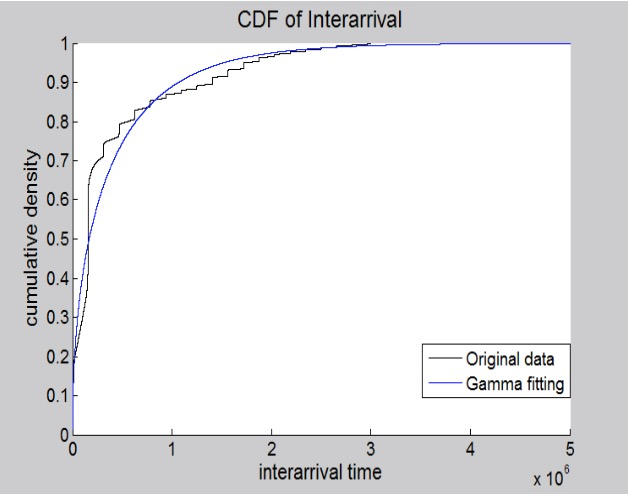
\includegraphics[scale=0.5]{write_gamma_cdf.png}
\end{center}
We can see from the above that the graph fits does for the empirical distribution. It is common cause gamma distribution is not a good fit for this.

\item[b.] 
Compare statistics of queuing when driving a FIFO queue.

After running the program, I got the result as below:
\begin{table}[htdp]
\caption{metric: Gamma verus Original}
\begin{center}
\begin{tabular}{c|c|c|c}
	& $\overline{d}$ & $\overline{q}$ & $\overline{x}$ \\
\hline
Gamma & 342.2 & 0.0002 & 0.00015 \\
\hline
Original &1413.7 & 0.00008 & 0.00015
\end{tabular}
\end{center}
\label{default}
\end{table}%
There is a big difference from Gamma and Original trace, so we can conclude Gamma is not a good fit for this one.
\end{enumerate}

\subsubsection{Exponential Distribution}
%Exponential
\begin{enumerate}
\item[a.]
Using MLE we find that $u=17085318$ and we can get the exponential distribution based on that. Then we can plot the graph as below:
\begin{center}
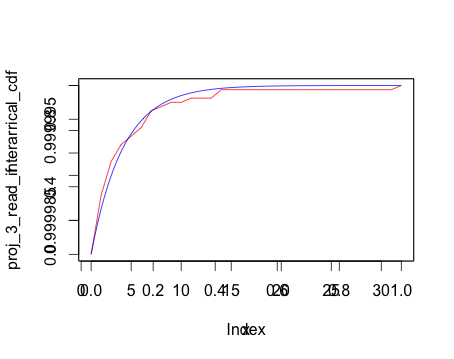
\includegraphics[scale=0.5]{write_exp_cdf.png}
\end{center}
From the graph above, we can easily see that the result is much better than the Gamma one.



\item[b.]
Compare statistics of queuing when drive a FIFO queue.
\begin{table}[htdp]
\caption{metric: Exponential verus Original}
\begin{center}
\begin{tabular}{c|c|c|c}
	& $\overline{d}$ & $\overline{q}$ & $\overline{x}$ \\
\hline
Exponential & 0.2942 & 1.7e-8 & 0.00015 \\
\hline
Original &1413.7 & 0.00008 & 0.00015
\end{tabular}
\end{center}
\label{default}
\end{table}%
The difference on $\overline{q}$ is much closer though $\overline{d}$ is bigger, but the simulated fitted line is better than previous one.
\end{enumerate}
\subsubsection{Log linear Distribution}
%Log linear
\begin{enumerate}
\item[a.]
Applying MLE we can get $a=18.4484$, $b=3.5803$, then we can plot the two plots as below:
\begin{center}
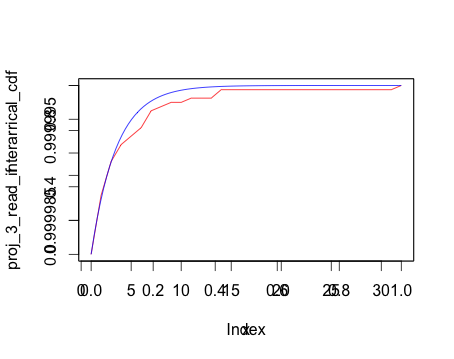
\includegraphics[scale=0.5]{write_log_cdf.png}
\end{center}
This one is also better than Gamma but not as good as the Exponential.


\item[b.]
Compare statistics when running a FIFO queue:
\begin{table}[htdp]
\caption{metric: log linear verus Original}
\begin{center}
\begin{tabular}{c|c|c|c}
	& $\overline{d}$ & $\overline{q}$ & $\overline{x}$ \\
\hline
Log linear & 22.41 & 0.0001 & 0.00015 \\
\hline
Original &1413.7 & 0.00008 & 0.00015
\end{tabular}
\end{center}
\label{default}
\end{table}%
\end{enumerate}

\subsection{Read Part}

%3 methods implement for read
\subsubsection{Gamma Distribution}
%Gamma
Applying MLE and we can get $a=0.222591$, $b=767565000$, the graph is also weird for the empirical data. The statistics of queuing is as below:
\begin{table}[htdp]
\caption{metric: Gamma verus Original}
\begin{center}
\begin{tabular}{c|c|c|c}
	& $\overline{d}$ & $\overline{q}$ & $\overline{x}$ \\
\hline
Gamma & 6981.4 & 0.017 & 0.05 \\
\hline
Original &3115.6 & 0.008 & 0.05
\end{tabular}
\end{center}
\label{default}
\end{table}% 
\\
We can see the difference between $\overline{d}$ is still big.
\subsubsection{Exponential Distribution}
%Exponential
Using MLE we can get $u=386178$, and the graph is similar to the Write part. The statistics of queuing is as below:
\begin{table}[htdp]
\caption{metric: Exponential verus Original}
\begin{center}
\begin{tabular}{c|c|c|c}
	& $\overline{d}$ & $\overline{q}$ & $\overline{x}$ \\
\hline
Gamma & 2235.3& 0.006 & 0.05 \\
\hline
Original &3115.6 & 0.008 & 0.05
\end{tabular}
\end{center}
\label{default}
\end{table}%
\\
Also, exponential seems to be the best fit for this trace.
\subsubsection{Log linear Distribution}
As above, we can using MLE to get $a=12.0341$, $b=1.93794$. The same method can be implemented and then we can get 
%Log linear
\begin{table}[htdp]
\caption{metric: Log Linear verus Original}
\begin{center}
\begin{tabular}{c|c|c|c}
	& $\overline{d}$ & $\overline{q}$ & $\overline{x}$ \\
\hline
Log Linear & 5134.2& 0.006 & 0.05 \\
\hline
Original &3115.6 & 0.008 & 0.05
\end{tabular}
\end{center}
\label{default}
\end{table}%
\\
Above all, I still think the exponential is the best fit for the trace $proj_3$.

\section{Question 3}
%Treat two classy as a single class one
Yes of course. From the data set above, we can see the fitted plot is almost the same result for read and write. Also, there is just a single server, which means the server can only handle one read or one write at the same time. So there is no need to consider them separately. Just like Homework 2, we can think them together which is a easier way to do data analysis.
\section{Question 4}

\begin{enumerate}
\item[i.]
Using ssq4 and making some changes to it, we can deal with the SJF problems. Using the method of batch means with $k=64$ batches with each size 1024. we can get the confidence interval of this problem:
\begin{table}[htdp]
\caption{metric: Batch means}
\begin{center}
\begin{tabular}{c|c|c|c|c}
 $\overline{d}$ & $\overline{w}$ & $\overline{l}$& $ \overline{q} $ & $ \overline{x} $\\
\hline
(0.12282,0.13617) & (0.20311,0.21596)& (2.03001,2.17279) & (1.23333, 1.36667) & (0.97501,0.80788) \\

\end{tabular}
\end{center}
\label{default}
\end{table}% 
%simulate
\item[ii.]
Changing the code to FIFO just as Homework 2, we can get another confidence interval with 95\%:
\begin{table}[htdp]
\caption{metric: Batch means}
\begin{center}
\begin{tabular}{c|c|c|c|c}
 $\overline{d}$ & $\overline{w}$ & $\overline{l}$& $ \overline{q} $ & $ \overline{x} $\\
\hline
(0.19287,0.22117) & (0.27331,0.30101)& (2.74444,3.07321) & (1.94409, 2.26011) & (0.79803,0.81410) \\

\end{tabular}
\end{center}
\label{default}
\end{table}% 
\item[iii.]
For this question, we need to have $\lambda < \mu$, and we can see all the result satisfies this constraint. So I believe my answer is the right answer for this question.
\item[iv.]
So I use hist\$density to draw the histograms of the waiting queue lengths for the two queues as below: \\
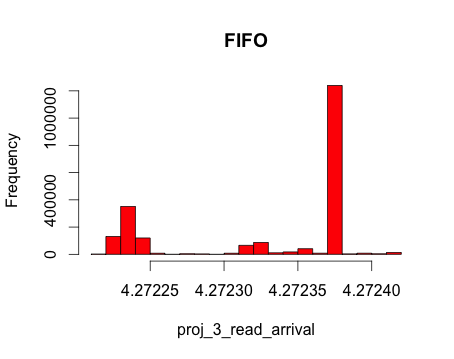
\includegraphics[scale=0.5]{FIFO_writing.png}
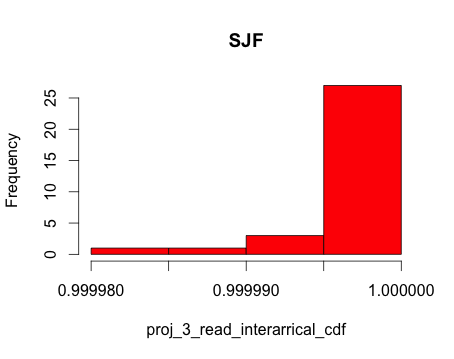
\includegraphics[scale=0.5]{SJF_waiting.png} \\
Obviously, we can get the waiting queue length time is less than the waiting queue length of FIFO since the length is from (0,2) in SJF comparing with (0,4) in FIFO.

\item[v.]
When comparing, we can see that SJF is better. I think the main reason is because that there are some huge jobs in the queue which causes FIFO waiting queue becomes longer. It is the same as why exponential is better than others since others may have more chance of getting huge jobs.
\end{enumerate}
\section{Question 5}
%repeat
From Homework 2, it is known that $proj_3$ is a good trace cause the autocorrelation is smooth, so I choose the $wdev_0$ trace to solve this problem.
\begin{enumerate}
\item[i.]
I will also use Erlang(4,0.02) random variable as service time. With $k=64$ and $b=1024$.
\begin{table}[htdp]
\caption{metric: Batch means}
\begin{center}
\begin{tabular}{c|c|c|c|c}
 $\overline{d}$ & $\overline{w}$ & $\overline{l}$& $ \overline{q} $ & $ \overline{x} $\\
\hline
$(5.92,11.34)10^8$ & $(5.81,11.23)10^8$& $(300,780)$ & $(300, 780)$ & $(0.2,0.3) $\\

\end{tabular}
\end{center}
\label{default}
\end{table}% 
\item[ii.]
Using FIFO we can get
\begin{table}[htdp]
\caption{metric: Batch means}
\begin{center}
\begin{tabular}{c|c|c|c|c}
 $\overline{d}$ & $\overline{w}$ & $\overline{l}$& $ \overline{q} $ & $ \overline{x} $\\
\hline
$(6.11,12.34)10^8$ & $(5.81,11.23)10^8$& $(300,780)$ & $(303, 780)$ & $(0.2,0.3) $\\

\end{tabular}
\end{center}
\label{default}
\end{table}% 
\item[iii.]
Also we need $\lambda < \mu$ and all the metrics are satisfied.
\item[iv.] 
Applying the same step as Question 4, we can get \\
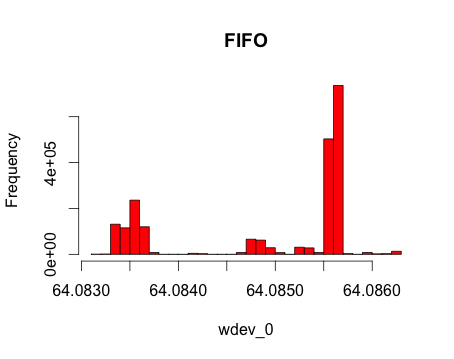
\includegraphics[scale=0.5]{1_1.png}
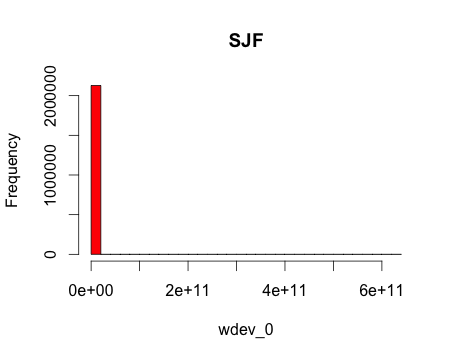
\includegraphics[scale=0.5]{1_2.png}
\item[v.]
I think for this trace, the answer is not very obvious. But I do not find a good $k$ for this problem, I think if the $k$ is suitable, the answer will be easy to figure out. Also when the batch increase, it should be accurate but when drawing histogram, we may need to drop some data.
\end{enumerate}

\end{document}
